\ifbook{

}

\ifslide {
 \section{Foreword}

 \begin{frame}
   \begin{block}{Some pratical details}
     \begin{itemize}
       \item I have previous experience in teaching, but to \textbf{technical} people or student
       \begin{itemize}
         \item ... so \textit{stop} me, if I go too fast !
       \end{itemize}
       \item I'm French, but I teach in \textbf{English} because my \textit{Deutsch ist schrecklich}
       \item Session last 3 hours, and are divided into:
       \begin{itemize}
         \item 15 minuten: small MCQ (Multiple choice questionnaire), starting next week
         \item ~1 hour
         \item 30" break
         \item ~1 hour
         \item 15" buffer if we are late or need to go deeper
       \end{itemize}
       \item we are here to \textbf{interact}, not to get your ears used to crappy english spoken by
       French people...
     \end{itemize}
   \end{block}
  \end{frame}


  \begin{frame}
    \begin{block}{Goals}
      \begin{itemize}
        \item Basic understanding of how and why program
        \item Impact in \textbf{your} job
        \item Enhance your communication skills with technical people
      \end{itemize}
    \end{block}

    \begin{block}{Who are you ?}
      \begin{itemize}
        \item Quickly gives us an hint of you are and where you come from...
      \end{itemize}
    \end{block}
  \end{frame}

  % classe outline
  \section{How computer works ?}

  \begin{frame}
    \begin{center}
        What do you know about \textbf{how} a computer work ?
    \end{center}
  \end{frame}

  \begin{frame}
   \begin{center}
     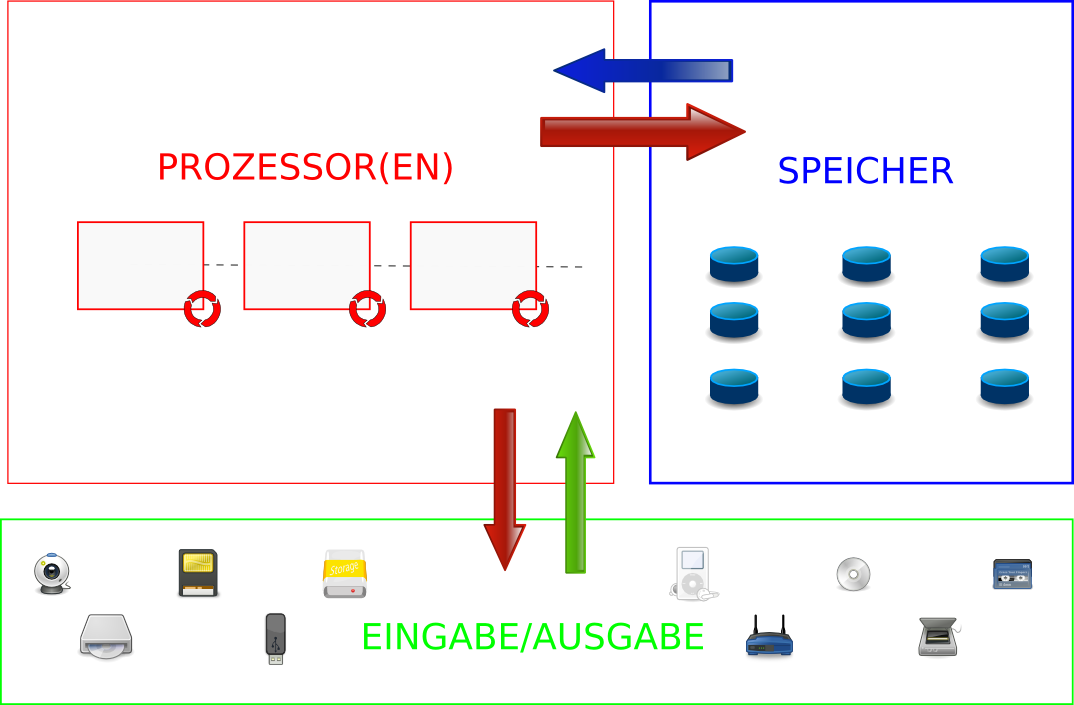
\includegraphics[scale=0.3]{img/cpu-schematics.png}
   \end{center}
  \end{frame}

  \begin{frame}
    \begin{center}
      \begin{itemize}
        \item What is an \textbf{operating system}(OS) ?
        \item Name a few OS names that you know of ?
        \item What does exactly an operating system ? What are its \textbf{responsabilities}?
      \end{itemize}
    \end{center}
  \end{frame}

  \begin{frame}{Role of an Operating System}
    \begin{center}
      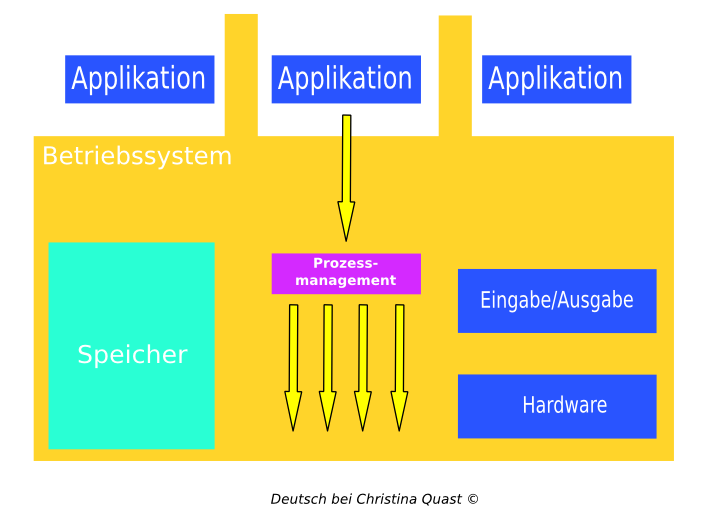
\includegraphics[scale=0.3]{img/operating-system.png}
    \end{center}
  \end{frame}

  \begin{frame}{Speed of I/Os}
    \begin{center}
      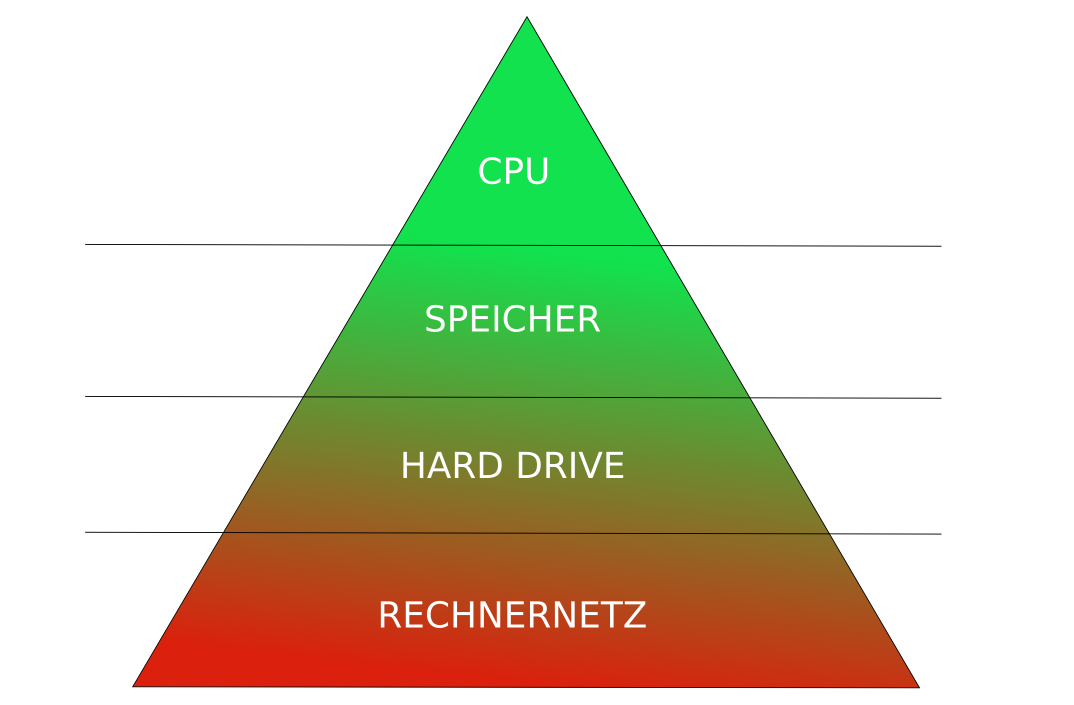
\includegraphics[scale=0.3]{img/pyramid-io.png}
    \end{center}
  \end{frame}

  \begin{frame}{First era of IT: Mainframe and terminals}
    \begin{center}
      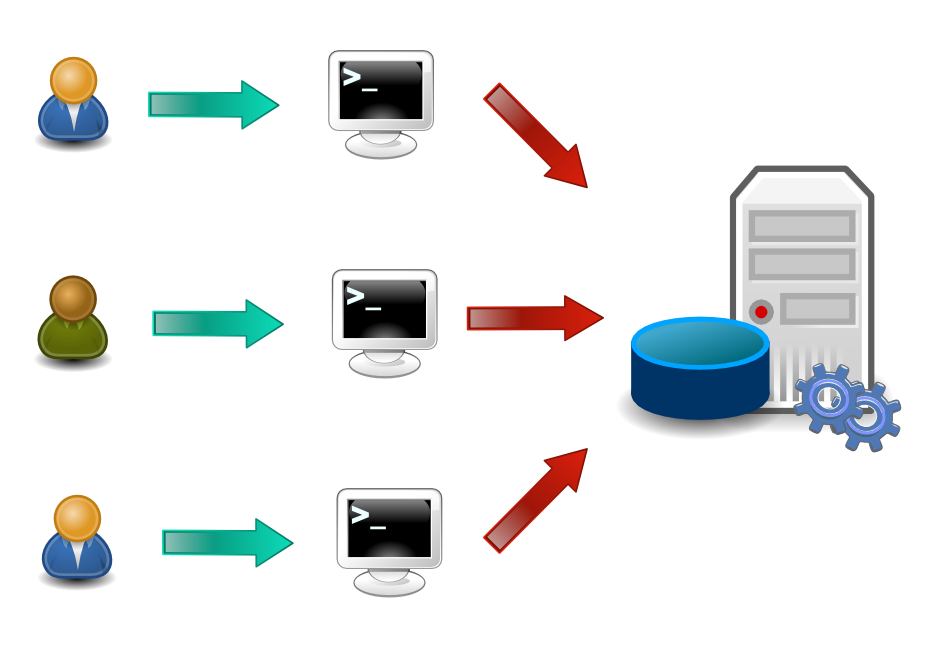
\includegraphics[scale=0.3]{img/mainframe-terminals.png}
    \end{center}
  \end{frame}

  \begin{frame}{Second era of IT: Clients and servers}
    \begin{center}
      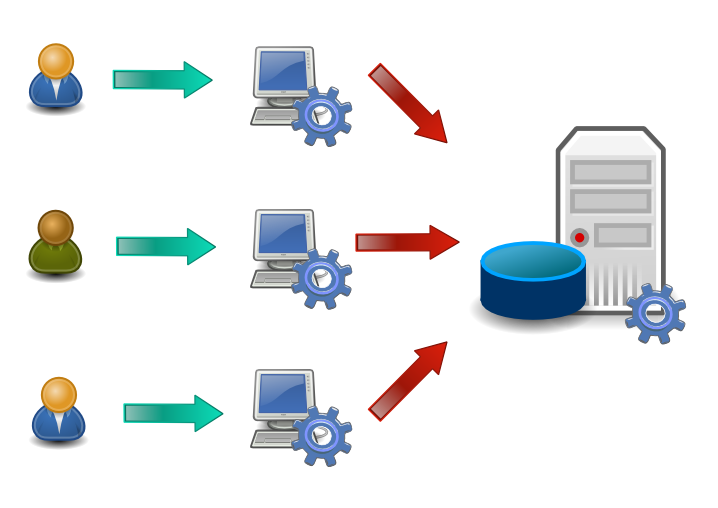
\includegraphics[scale=0.3]{img/fat-clients.png}
    \end{center}
  \end{frame}

  \begin{frame}{Third era of IT: The Internet}
    \begin{center}
      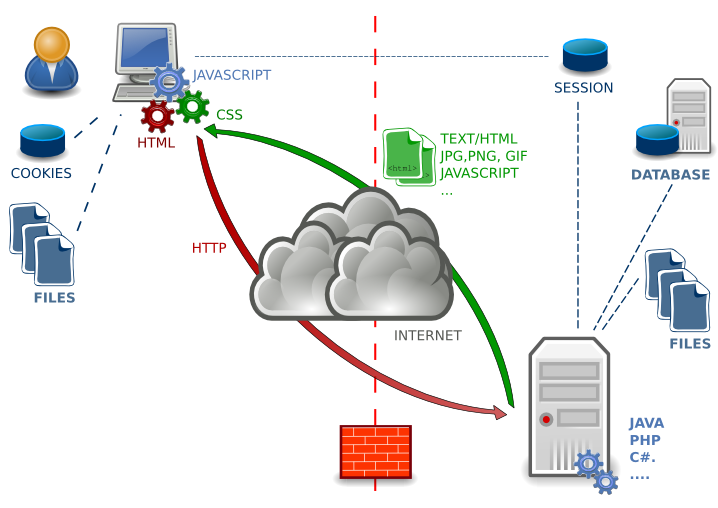
\includegraphics[scale=0.3]{img/internet.png}
    \end{center}
  \end{frame}

  \begin{frame}{Data persistance}
    \begin{center}
      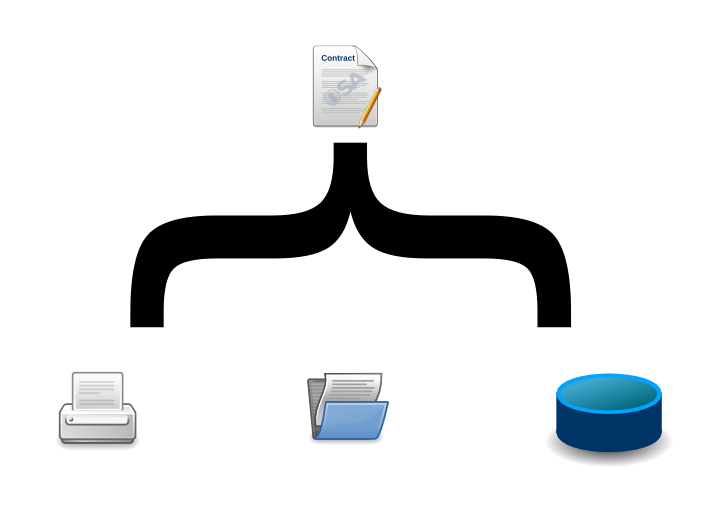
\includegraphics[scale=0.3]{img/persistance.png}
    \end{center}
  \end{frame}

  % TODO : Java and JVM

  % TD: Manually compile and run a HelloWorld
  % Bonus: Args ?

}
